\documentclass[11pt]{article}
\usepackage[utf8]{inputenc}
\usepackage[T1]{fontenc}
\usepackage{geometry, tikz, xcolor, enumitem, ragged2e}
\geometry{a4paper, margin=1.5cm}

\begin{document}

\begin{center}
\Large \textbf{\textcolor{green!50!black}{Atividade Remota: Cultura Digital – Mídias Digitais e Segurança Digital}}\\[0.3cm]
\large Professor: Jefferson
\end{center}

\vspace{0.3cm}
\large Nome: \underline{\hspace{8cm}} \quad Turma: \underline{\hspace{3cm}}

\vspace{0.5cm}

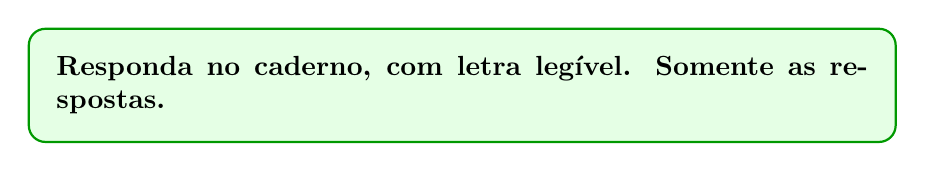
\begin{tikzpicture}
\node[rectangle, fill=green!10, rounded corners=6pt, inner sep=10pt, draw=green!60!black, thick]{
\begin{minipage}{0.85\linewidth}
\textbf{Responda no caderno, com letra legível. Somente as respostas.}
\end{minipage}
};
\end{tikzpicture}

\vspace{0.6cm}

\begin{enumerate}
\item O que são mídias digitais e como elas influenciam nossa vida diária?\\[1em]
\rule{\linewidth}{0.4pt}\\[1em]\rule{\linewidth}{0.4pt}\\[1em]\rule{\linewidth}{0.4pt}\\[1em]\rule{\linewidth}{0.4pt}\\[1em]\rule{\linewidth}{0.4pt}\\[1em]\rule{\linewidth}{0.4pt}\\[1em]\rule{\linewidth}{0.4pt}\\[1em]\rule{\linewidth}{0.4pt}

\item Explique o que é segurança digital e sua importância no uso da internet.\\[1em]
\rule{\linewidth}{0.4pt}\\[1em]\rule{\linewidth}{0.4pt}\\[1em]\rule{\linewidth}{0.4pt}\\[1em]\rule{\linewidth}{0.4pt}\\[1em]\rule{\linewidth}{0.4pt}\\[1em]\rule{\linewidth}{0.4pt}\\[1em]\rule{\linewidth}{0.4pt}\\[1em]\rule{\linewidth}{0.4pt}

\item Quais cuidados devem ser tomados ao compartilhar informações pessoais online?\\[1em]
\rule{\linewidth}{0.4pt}\\[1em]\rule{\linewidth}{0.4pt}\\[1em]\rule{\linewidth}{0.4pt}\\[1em]\rule{\linewidth}{0.4pt}\\[1em]\rule{\linewidth}{0.4pt}\\[1em]\rule{\linewidth}{0.4pt}\\[1em]\rule{\linewidth}{0.4pt}\\[1em]\rule{\linewidth}{0.4pt}

\item O que é um vírus digital e como ele pode afetar um computador?\\[1em]
\rule{\linewidth}{0.4pt}\\[1em]\rule{\linewidth}{0.4pt}\\[1em]\rule{\linewidth}{0.4pt}\\[1em]\rule{\linewidth}{0.4pt}\\[1em]\rule{\linewidth}{0.4pt}\\[1em]\rule{\linewidth}{0.4pt}\\[1em]\rule{\linewidth}{0.4pt}\\[1em]\rule{\linewidth}{0.4pt}

\item Por que é importante usar senhas fortes e diferentes em cada conta?\\[1em]
\rule{\linewidth}{0.4pt}\\[1em]\rule{\linewidth}{0.4pt}\\[1em]\rule{\linewidth}{0.4pt}\\[1em]\rule{\linewidth}{0.4pt}\\[1em]\rule{\linewidth}{0.4pt}\\[1em]\rule{\linewidth}{0.4pt}\\[1em]\rule{\linewidth}{0.4pt}\\[1em]\rule{\linewidth}{0.4pt}

\item Como identificar uma fake news nas redes sociais?\\[1em]
\rule{\linewidth}{0.4pt}\\[1em]\rule{\linewidth}{0.4pt}\\[1em]\rule{\linewidth}{0.4pt}\\[1em]\rule{\linewidth}{0.4pt}\\[1em]\rule{\linewidth}{0.4pt}\\[1em]\rule{\linewidth}{0.4pt}\\[1em]\rule{\linewidth}{0.4pt}\\[1em]\rule{\linewidth}{0.4pt}

\item O que é ciberbullying e como podemos combatê-lo?\\[1em]
\rule{\linewidth}{0.4pt}\\[1em]\rule{\linewidth}{0.4pt}\\[1em]\rule{\linewidth}{0.4pt}\\[1em]\rule{\linewidth}{0.4pt}\\[1em]\rule{\linewidth}{0.4pt}\\[1em]\rule{\linewidth}{0.4pt}\\[1em]\rule{\linewidth}{0.4pt}\\[1em]\rule{\linewidth}{0.4pt}

\item Cite boas práticas para manter a segurança digital em casa e na escola.\\[1em]
\rule{\linewidth}{0.4pt}\\[1em]\rule{\linewidth}{0.4pt}\\[1em]\rule{\linewidth}{0.4pt}\\[1em]\rule{\linewidth}{0.4pt}\\[1em]\rule{\linewidth}{0.4pt}\\[1em]\rule{\linewidth}{0.4pt}\\[1em]\rule{\linewidth}{0.4pt}\\[1em]\rule{\linewidth}{0.4pt}

\end{enumerate}

\end{document}

